\section{Età della vegetazione nelle isole}
Utilizzando le mappe del cambiamento esperito dalle isole si possono ottenere mappe che indicano un'età approssimativa della vegetazione che compone queste isole. 
\\
L'ipotesi che si vuole verificare è che sia la vegetazione più giovane quella ad essere maggiormente erosa in quanto può essere divelta più facilmente.
Non si esclude tuttavia di osservare erosione anche di vegetazione matura poiché le isole poste in corrispondenza dell'estradosso di un canale in curva sono soggette a scavo laterale.

\subsection{Metodi: estendere i confronti e ottenere un'età}
\paragraph{Limiti}
Con le immagini satellitari utilizzate non è possibile distinguere i singoli alberi che compongono le isole; se con le immagini a miglior risoluzione si distinguono gli arbusti isolati, non si può certo ottenere una stima dell'età tanto precisa quanto quella fornita da un carotaggio del tronco.
In più, una cella è classificata come vegetazione solo quando le piante al suo interno presentano complessivamente una chioma sufficientemente grande da occupare gran parte della cella; pertanto le immagini con celle di \SI{10}{\m} o  \SI{15}{\m} non possono mostrare che grandi macchie di vegetazione.
Prima dei \SI{3}{\anni} una pianta di salice generalmente non ha fronde molto estese.
\\
Occorre poi tenere in conto che le piante crescono differentemente in base alle condizioni ambientali: periodi di stress idrico o termico rallentano la crescita, così come il parziale seppellimento con ghiaia dovuto ad eventi di piena; una falda non troppo profonda la cui altezza varia lentamente, terreno di granulometria sottile con sabbia e buone temperature sono invece fattori favorevoli alla crescita \squarecite{Gurnell:2001-island-formation}.

Si crede che ciò che possa generalmente accadere è che fino ad una certa età, circa \SI{3}{\anni}, la nuova vegetazione non sia visibile dal satellite; quindi si può definire come età della vegetazione presente in una cella la somma della persistenza (il periodo di tempo in cui si osserva che la cella rimane vegetata) con i \SI{3}{\anni} iniziali. 

Le mappe del cambiamento sono state ottenute dalle mappe di classificazione; non essendo le seconde correttamente georeferenziate, neanche le prime lo sono. L'errore residuo nel processo di correzione è di 1~cella.

Infine, per poter confrontare nel corso degli anni ogni cella, le mappe del cambiamento sono state ricampionate alla risoluzione più bassa, corrispondente a celle di~\SI{15}{\m} di lato. Si è proceduto come mostrato nel paragrafo \ref{par:camb-limiti} ottenendo sempre valori $RSQR < \SI{1.5}{\percent}$; i confronti a~\SI{10}{\m} sono stati ricampionati a~\SI{15}{\m} applicando il valore del $75_\mathrm{mo}$ percentile (terzo quartile).
 

%TODO le piante crescono diversamente in base alle condizioni ambientali (cita articolo Gurnell?) → definire un'età in base al tempo di osservazione è un approccio limitato (qualche altro lavoro simile)

\paragraph{Obiettivo ed approccio} 
Date le precedenti premesse, bisogna riflettere su ciò che si vuole ottenere: dividere la vegetazione in classi di età.
Si vuole sapere quanta vegetazione giovane è stata erosa; non conta se questa ha esattamente \SI{3}{\anni} o \SI{4}{\anni}, l'importante è che sia grossomodo classificata come giovane.

Ogni mappa del cambiamento è formata dalle informazioni contenute in due mappe: quella più vecchia e quella più recente. La distanza temporale tra queste due mappe definisce il periodo di osservazione.
\\
Per la mappa del cambiamento più vecchia (la prima mappa di confronto in \vref{tab:confronti}), l'età della vegetazione delle isole è stata scelta essere pari al periodo di osservazione, cui si sono aggiunti \SI{3}{\anni}, che è ritenuto il periodo minimo affinché un insieme di piante diventi visibile per il satellite.
\\
Per le mappe via via più recenti, l'età nelle celle delle isole che non sono cambiate è pari al periodo di osservazione sommato all'età precedente; per le celle si sono vegetate a partire dall'alveo l'età è pari al periodo di osservazione con l'aggiunta di \SI{3}{\anni}.

L'approccio di definire un'età in base al periodo di osservazione è limitato, in particolare per le mappe più vecchie, poiché non è possibile tener conto della vegetazione che era presente antecedentemente alla prima immagine valida;
si ritiene che a partire dalla $4^a$ o $5^a$ mappa di età il metodo inizi ad essere affidabile (generalmente quindi dalla mappa di età del 2007-09-21).
Per gli scopi della ricerca questo approccio risulta essere sufficiente.

\medskip
Si osservino i grafici in \vref{graph:distrib-rapp-eros-eta}, i quali rappresentano quante isole sono state erose rispetto alle isole presenti in ogni tratto in base all'età delle prime.
Si vede come le isole con età minore di \SI{5}{\anni} siano spesso erose; si evidenzia anche una dinamicità per le isole con età tra \SIrange[range-phrase={ e }]{5}{8}{\anni}. 
\\
Si definiscono quindi le seguenti classi di età:
%
\begin{itemize}
	\item giovane, con meno di \SI{5}{\anni};
	\item intermedia, con età compresa tra \SIrange[range-phrase={ e }]{5}{8}{\anni};
	\item matura, con più di \SI{8}{\anni}.
\end{itemize}
%
\begin{figure}
	\centering
	\tikzsetnextfilename{rapp_eros_eta}
\begin{tikzpicture}
	\begin{groupplot}[
		group style = {
			group size = 2 by 3,
			y descriptions at = edge left,
			x descriptions at = edge bottom,
			horizontal sep = 0.4cm,
			vertical sep = 0.4cm,
		},
		width = 0.54\textwidth,
		height = 0.54\textwidth,
		xlabel = {Età \si{[\anni]}},
		xmin = 3,
		xmax = 20,
		xtick distance = 3,
		enlarge x limits = 0.05,
		ylabel = {Isole erose / isole totali \si{[\percent]}},
		boxplot/draw direction = y,
		ymax = 70,
		ymin = 0,
		enlarge y limits = 0.05,
		grid = major,
	]
	\nextgroupplot % ASTER 2008_07_05
		\addplot [only marks]
			table [x=Eta, y=Perc_erosa_su_tot_isole] {graphics/data/rapp_eros_eta_2008_07_05.txt};
		\addplot [no markers, dashed, red]
			coordinates{(5,0) (5,70)};
		\addplot [no markers, dashed, red]
			coordinates{(8,0) (8,70)};
        \node [fill = white, draw = black, anchor = north east] 
        	at (axis description cs: 1,1) {AST 2008-07-05};
	%------------------------------------------------------
	\nextgroupplot % ASTER 2010_09_29
		\addplot [only marks]
			table [x=Eta, y=Perc_erosa_su_tot_isole] {graphics/data/rapp_eros_eta_2010_09_29.txt};
		\addplot [no markers, dashed, red]
			coordinates{(5,0) (5,70)};
		\addplot [no markers, dashed, red]
			coordinates{(8,0) (8,70)};
        \node [fill = white, draw = black, anchor = north east] 
        	at (axis description cs: 1,1) {AST 2010-09-29};
	%------------------------------------------------------
	\nextgroupplot % ASTER 2014_09_08
		\addplot [only marks]
			table [x=Eta, y=Perc_erosa_su_tot_isole] {graphics/data/rapp_eros_eta_2014_09_08.txt};
		\addplot [no markers, dashed, red]
			coordinates{(5,0) (5,70)};
		\addplot [no markers, dashed, red]
			coordinates{(8,0) (8,70)};
        \node [fill = white, draw = black, anchor = north east] 
        	at (axis description cs: 1,1) {AST 2014-09-08};
	%------------------------------------------------------
	\nextgroupplot % Sentinel2 2015_09_12
		\addplot [only marks]
			table [x=Eta, y=Perc_erosa_su_tot_isole] {graphics/data/rapp_eros_eta_2015_09_12.txt};
		\addplot [no markers, dashed, red]
			coordinates{(5,0) (5,70)};
		\addplot [no markers, dashed, red]
			coordinates{(8,0) (8,70)};
        \node [fill = white, draw = black, anchor = north east] 
        	at (axis description cs: 1,1) {S2 2015-09-12};
	%------------------------------------------------------
	\nextgroupplot % Sentinel2 2015_10_22
		\addplot [only marks]
			table [x=Eta, y=Perc_erosa_su_tot_isole] {graphics/data/rapp_eros_eta_2015_10_22.txt};
		\addplot [no markers, dashed, red]
			coordinates{(5,0) (5,70)};
		\addplot [no markers, dashed, red]
			coordinates{(8,0) (8,70)};
        \node [fill = white, draw = black, anchor = north east] 
        	at (axis description cs: 1,1) {S2 2015-10-22};
	%------------------------------------------------------
	\nextgroupplot % Sentinel2 2017_06_13
		\addplot [only marks]
			table [x=Eta, y=Perc_erosa_su_tot_isole] {graphics/data/rapp_eros_eta_2017_06_13.txt};
		\addplot [no markers, dashed, red]
			coordinates{(5,0) (5,70)};
		\addplot [no markers, dashed, red]
			coordinates{(8,0) (8,70)};
        \node [fill = white, draw = black, anchor = north east] 
        	at (axis description cs: 1,1) {S2 2017-06-13};
	\end{groupplot}
\end{tikzpicture}

	\caption[distribuzione del rapporto tra isole erose e la somma delle isole presenti]{distribuzione del rapporto tra le isole erose e la sommatoria di tutte le isole presenti per ogni tratto nei tratti da \numrange[range-phrase={ a }, mode=text]{1}{23} in base all'età; le linee verticali rosse tratteggiate indicano l'età di \SIrange[range-phrase={ e }]{5}{8}{\anni}.}
	\label{graph:distrib-rapp-eros-eta}
\end{figure}

\paragraph{Validazione}
Da un controllo visuale delle mappe di età si vede una corrispondenza tra struttura dell'età in diversi tipi di isole e quanto osservato da rilievi e osservazioni in campo \squarecite{Gurnell:2001-island-formation}: le isole complesse hanno una struttura d'età a macchie, quelle distaccate da floodplain uniforme (\vref{fig:struttura-eta}).
%
\begin{figure}
	\centering
	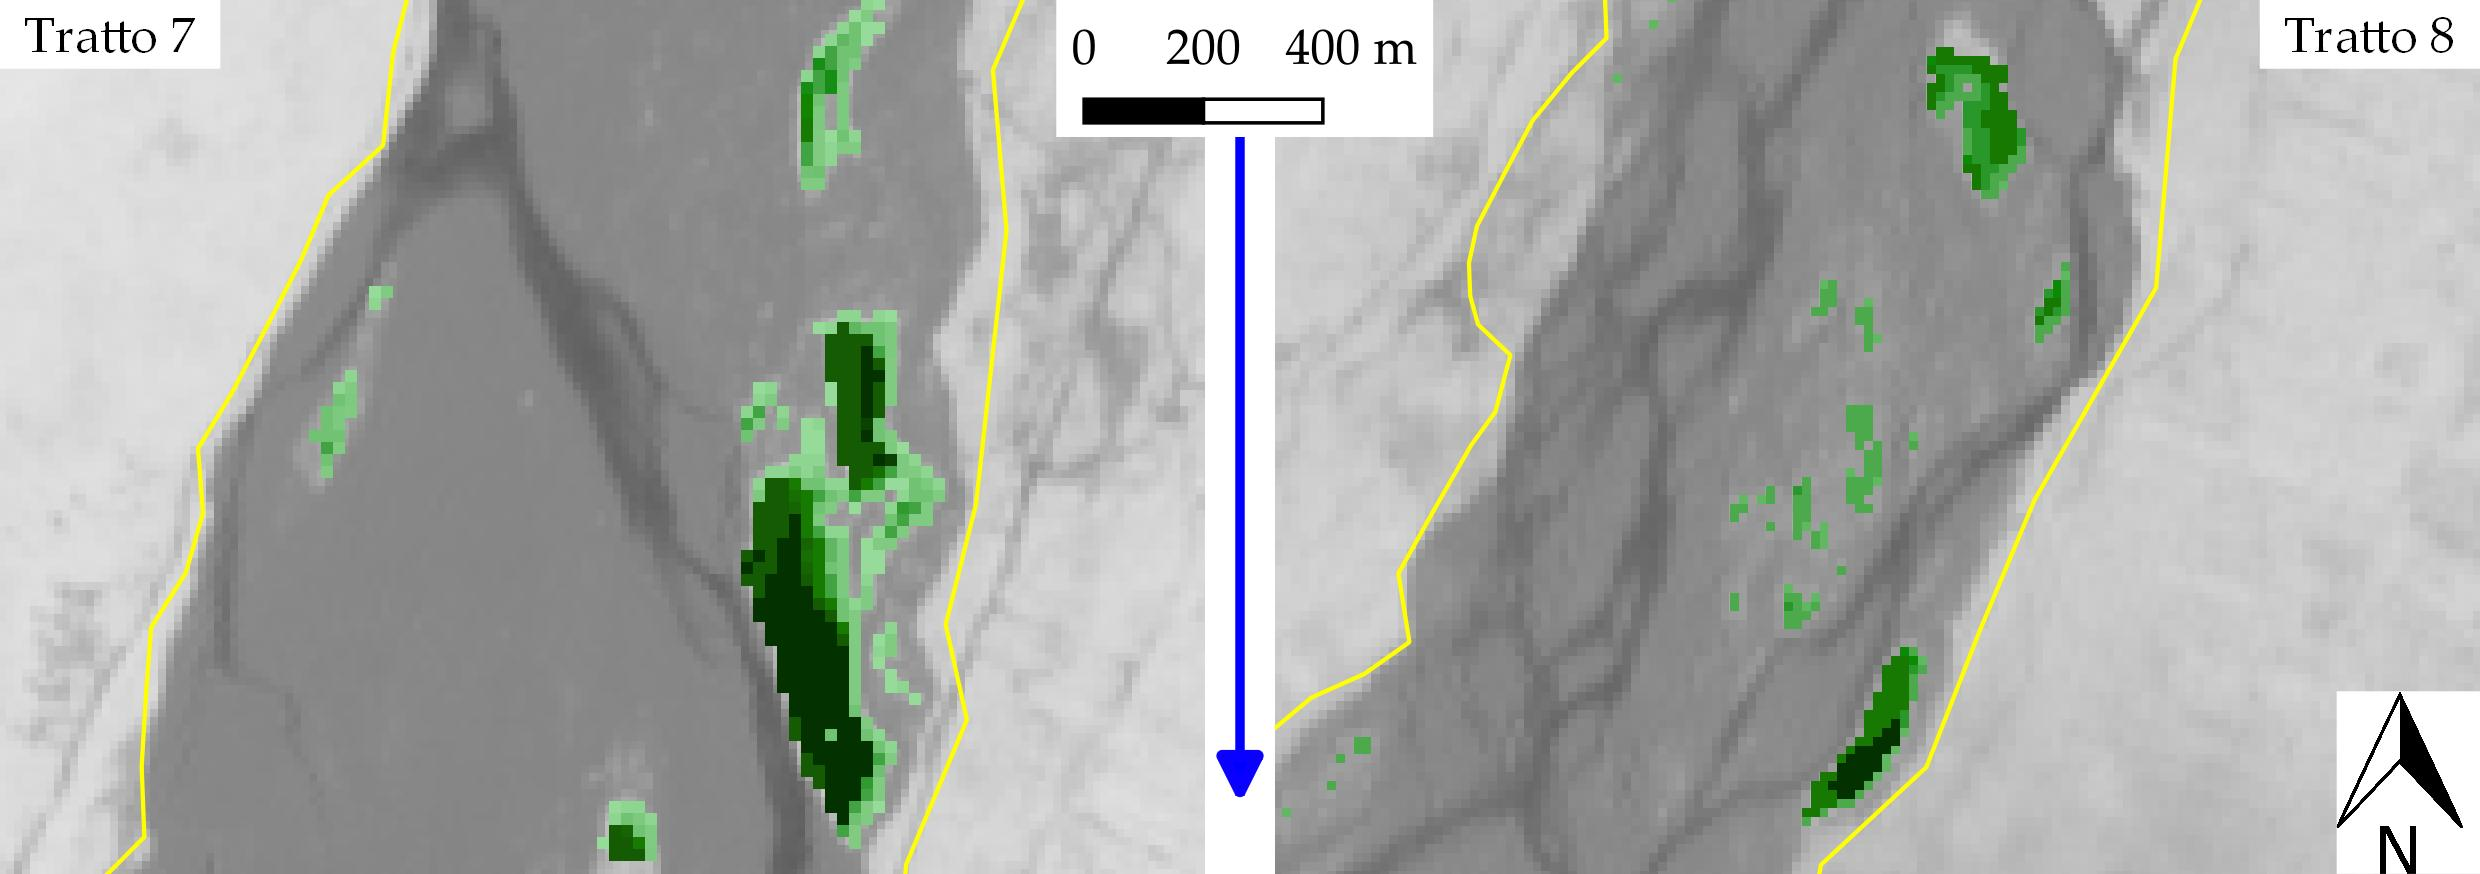
\includegraphics[width = \textwidth]{files/struttura_eta.jpeg}
	\caption[mappe della struttura di età in due tratti]{mappe della struttura di età in due tratti; i colori più scuri indicano una maggiore età.
		Nel tratto~7 (2017-06-13) si vede la struttura a macchie dell'età della vegetazione nelle isole complesse;
		nel tratto~8 (2009-07-08) si osserva la distribuzione più unifome dell'età nell'isola in basso, che si è formata dalla \emph{floodplain}.
		La maschera computazionale è mostrata in giallo; sullo sfondo sono mostrate le mappe NDVI.}
	\label{fig:struttura-eta}
\end{figure}
%

Il CHM (\emph{Canopy Height Model}) è il modello digitale della copertura arborea; similmente al DEM, mostra delle quote; queste sono tuttavia riferite all'altezza della vegetazione sopra il terreno.
\\
È generalmente sensato affermare che piante più mature abbiano un'altezza maggiore di piante giovani.
Quindi si sono utilizzati i dati di altezza della copertura arborea contenuti nei CHM di agosto~2010 e del~2013-10-22 per verificare che nelle celle della mappa di età della vegetazione rispettivamente del~2010-09-29 e del~2013-09-05 l'altezza fosse all'incirca proporzionale all'età.
Tra le date di ottenimento dei CHM e delle immagini \AST{} non vi sono stati eventi idrologici rilevanti.
I CHM sono stati ricampionati a \SI{15}{\m} (larghezza delle celle delle immagini \AST{}) applicando il valore del $75_{\mathrm{mo}}$ percentile in quanto rappresenta l'altezza delle chiome più elevate ed espanse, le quali dovrebbero definire i valori di età nelle mappe essendo maggiormente visibili da satellite.
\\
Si è scelto di validare la procedura solo sulle mappe di età del~2010 e del~2013 poiché sono più rappresentative della reale distribuzione d'età delle piante, mentre la mappa di età del 2005-08-30 potrebbe non essere affidabile per quanto precedentemente esposto.
\\
I \emph{boxplot} della distribuzione dell'altezza della vegetazione rispetto all'età sono presentati nel grafico in \vref{graph:altezza-chm-eta}.
Il loro andamento crescente riflette sufficientemente quello dei dati da rilievi dendrometrici effettuati da \squarecite{Gurnell:2018-canopy-height} su isole pioniere nel Tagliamento localizzate nei medesimi tratti del CHM; pertanto ci si ritiene soddisfatti della procedura sviluppata in quanto riesce ad ottenere una stima dell'età delle piante nelle isole adeguata agli scopi della tesi.
%
\begin{figure}
	\centering
	\tikzsetnextfilename{percentili_CHM_eta}
\begin{tikzpicture}
	\begin{groupplot}[
		group style = {
			group size = 3 by 1,
			y descriptions at = edge left,
			x descriptions at = edge bottom,
			horizontal sep = 0.3cm,
			vertical sep = 0.1cm,
		},
		width = 0.38\textwidth,
		height = 0.4\textwidth,
		xlabel = {Età \si{[\anni]}},
		xticklabel style = {font=\tiny},
		ylabel = {Altezza della chioma \si{[\m]}},
		boxplot/draw direction = y,
		ymax = 25,
		ymin = 0,
		enlarge y limits = 0.05,
		grid = major,
	]
	\nextgroupplot[
		xtick = {1, 2, 3, 4, 5, 6},
		xticklabels = {$4$, $5$, $6$, $7$, $9$, $13$},
		] % CSM età 2010
		\addplot [
			boxplot prepared = {
				lower whisker=0.44979499999999994,
				lower quartile=0.706821,
				median=1.349386,
				upper quartile=2.248977,
				upper whisker=3.919646,
				}
			]
			coordinates{};
		\addplot [
			boxplot prepared = {
				lower whisker=0.578308,
				lower quartile=0.963847,
				median=2.37749,
				upper quartile=4.048159,
				upper whisker=5.461802,
				}
			]
			coordinates{};
		\addplot [
			boxplot prepared = {
				lower whisker=0.706821,
				lower quartile=1.349386,
				median=2.634516,
				upper quartile=4.819237,
				upper whisker=8.700328600000006,
				}
			]
			coordinates{};
		\addplot [
			boxplot prepared = {
				lower whisker=0.9252931000000002,
				lower quartile=1.51002725,
				median=2.37749,
				upper quartile=4.0160307500000005,
				upper whisker=7.5951168,
				}
			]
			coordinates{};
		\addplot [
			boxplot prepared = {
				lower whisker=1.349386,
				lower quartile=2.634516,
				median=6.361392,
				upper quartile=11.244886,
				upper whisker=17.156482,
				}
			]
			coordinates{};
		\addplot [
			boxplot prepared = {
				lower whisker=4.94775,
				lower quartile=9.3814475,
				median=14.200684,
				upper quartile=19.341203,
				upper whisker=23.350807599999996,
				}
			]
			coordinates{};
		\node [fill = white, draw = black, anchor = north west] 
        	at (axis description cs: 0,1) {2010};
	%------------------------------------------------------
	\nextgroupplot[
		xtick = {1, 2, 3, 4, 5, 6, 7, 8, 9, 10},
		xticklabels = {$4$, $6$, $7$, $8$, $9$, $10$, $11$, $12$, $14$, $16$},
		] % CSM età 2013
		\addplot [
			boxplot prepared = {
				lower whisker=0.304544,
				lower quartile=0.657206,
				median=1.597636,
				upper quartile=3.713603,
				upper whisker=6.1352108000000065,
				}
			]
			coordinates {};
		\addplot [
			boxplot prepared = {
				lower whisker=0.774759,
				lower quartile=1.244974,
				median=2.420512,
				upper quartile=3.831157,
				upper whisker=5.594463,
				}
			]
			coordinates {};
		\addplot [
			boxplot prepared = {
				lower whisker=1.244974,
				lower quartile=1.950297,
				median=3.360942,
				upper quartile=5.006695,
				upper whisker=6.770001,
				}
			]
			coordinates {};
		\addplot [
			boxplot prepared = {
				lower whisker=1.6211462,
				lower quartile=3.125835,
				median=5.006695,
				upper quartile=7.122662,
				upper whisker=9.4972484,
				}
			]
			coordinates {};
		\addplot [
			boxplot prepared = {
				lower whisker=1.950297,
				lower quartile=3.243388,
				median=4.654033,
				upper quartile=6.534893,
				upper whisker=8.262933799999999,
				}
			]
			coordinates {};
		\addplot [
			boxplot prepared = {
				lower whisker=2.65562,
				lower quartile=3.59605,
				median=5.124248,
				upper quartile=6.9169435,
				upper whisker=9.097565300000001,
				}
			]
			coordinates {};
		\addplot [
			boxplot prepared = {
				lower whisker=3.478496,
				lower quartile=4.71281,
				median=6.652447,
				upper quartile=9.4149605,
				upper whisker=12.2009848,
				}
			]
			coordinates {};
		\addplot [
			boxplot prepared = {
				lower whisker=2.65562,
				lower quartile=4.5952565,
				median=8.2982,
				upper quartile=12.706465999999999,
				upper whisker=17.608457000000005,
				}
			]
			coordinates {};
		\addplot [
			boxplot prepared = {
				lower whisker=3.125835,
				lower quartile=4.418926,
				median=8.592084,
				upper quartile=13.35301175,
				upper whisker=15.351425,
				}
			]
			coordinates {};
		\addplot [
			boxplot prepared = {
				lower whisker=6.570159200000001,
				lower quartile=11.3252095,
				median=15.351425,
				upper quartile=21.3760555,
				upper whisker=24.8027469,
				}
			]
			coordinates {};
		\node [fill = white, draw = black, anchor = north west] 
        	at (axis description cs: 0,1) {2013};
	%------------------------------------------------------
	\nextgroupplot[
		xtick = {1, 2, 3, 4},
		xticklabels = {$5$, $10$, $13$, $16$},
		]
		\addplot [
			boxplot prepared = {
				lower whisker=1.46,
				lower quartile=1.9,
				median=1.96,
				upper quartile=3.99,
				upper whisker=5.25,
				}
			]
			coordinates {};
		\addplot [
			boxplot prepared = {
				lower whisker=4.27,
				lower quartile=6.23,
				median=7.06,
				upper quartile=9.08,
				upper whisker=11.61,
				}
			]
			coordinates {};
		\addplot [
			boxplot prepared = {
				lower whisker=7.85,
				lower quartile=8.99,
				median=10.25,
				upper quartile=13.42,
				upper whisker=14.12,
				}
			]
			coordinates {};
		\addplot [
			boxplot prepared = {
				lower whisker=10.92,
				lower quartile=12.06,
				median=14.46,
				upper quartile=16.11,
				upper whisker=21.30,
				}
			]
			coordinates {};
		\node [fill = white, draw = black, anchor = north west] 
        	at (axis description cs: 0,1) {Gurnell et al. 2018};
	\end{groupplot}
\end{tikzpicture}

	\caption[distribuzione dell'altezza delle piante secondo l'età]{distribuzione dell'altezza delle piante (dal CHM) secondo l'età (dalle mappe di età) per il 2010 e il 2013 confrontati con rilievi dendrometrici presentati da \squarecite{Gurnell:2018-canopy-height}.}
	\label{graph:altezza-chm-eta}
\end{figure}
%

\subsection{Risultati: un trend per la vegetazione erosa}
Osservando la distribuzione del rapporto tra isole erose e isole presenti rispetto all'età, sono state definite 3~classi di età della vegetazione:
%
\begin{itemize}
	\item giovane, con meno di \SI{5}{\anni};
	\item intermedia, con età compresa tra \SIrange[range-phrase={ e }]{5}{8}{\anni};
	\item matura, con più di \SI{8}{\anni}.
\end{itemize}
%
Si considerino le isole presenti in alcuni tratti e alcune immagini divise per classi di età; si considerino anche le isole erose in seguito alle immagini di cui sopra, divise per classi di età e nei medesimi tratti: ciò che si vede nel grafico in \vref{graph:distr-eta} è la quantità di isole erose per ogni classe rispetto alle isole presenti. 
%
\begin{figure}
	\centering
	\tikzsetnextfilename{eta_tratti_8_11_17}
\begin{tikzpicture}
	\begin{groupplot}[
		group style = {
			group size = 3 by 1,
			x descriptions at = edge bottom,
			y descriptions at = edge left,
			xticklabels at = all,
			horizontal sep = 0.2cm,
			vertical sep = 0.25cm,
		},
		width = 0.37\textwidth,
		height = 0.8\textwidth,
	    xbar stacked,
		enlarge x limits = 0.02,
		enlarge y limits = 0.10,
		symbolic y coords = {
			2008-07-05, 2009-07-08, 
			2012-08-01, 2013-09-05,  
			2016-09-13, 2017-06-13
		},
		ytick distance = 1,
		%scaled x ticks = false,
		xlabel = {Areale \si{[\m\tothe{2}]}},
		xmajorgrids = true,
		]
		\nextgroupplot % tratto_8
			\addplot[bar shift = .4cm, pattern = north east lines]
		       	table [y=data, x=giovane-e] {graphics/data/tr_8_eta.txt};
			\addplot[bar shift = .4cm, fill = green]
		       	table [
		       		y=data, 
		       		x expr=\thisrow{giovane} - \thisrow{giovane-e}
		       		] {graphics/data/tr_8_eta.txt};
		       		
			\resetstackedplots
			\addplot[bar shift = 0cm, pattern = north east lines, forget plot]
		       	table [y=data, x=interm-e] {graphics/data/tr_8_eta.txt};
			\addplot[bar shift = 0cm, fill = green!75!black]
		       	table [
		       		y=data, 
		       		x expr=\thisrow{interm} - \thisrow{interm-e}
		       		] {graphics/data/tr_8_eta.txt};
		       		
			\resetstackedplots
			\addplot[bar shift = -.4cm, pattern = north east lines, forget plot]
		       	table [y=data, x=matura-e] {graphics/data/tr_8_eta.txt};
			\addplot[bar shift = -.4cm, fill = green!40!black]
		       	table [
		       		y=data, 
		       		x expr=\thisrow{matura} - \thisrow{matura-e}
		       		] {graphics/data/tr_8_eta.txt};
		    
        	\node [fill = white, draw = black, anchor = north east] 
        		at (axis description cs: 1,1) {Tr. 8};
        %
		\nextgroupplot [% tratto_11
			legend style = {
				at = {(0.5,1.02)},
				legend columns = 4,
				anchor = south
			}, 
			]
			\addplot[bar shift = .4cm, pattern = north east lines]
		       	table [y=data, x=giovane-e] {graphics/data/tr_11_eta.txt};
		    \addlegendentry{Erosione}
			\addplot[bar shift = .4cm, fill = green]
		       	table [
		       		y=data, 
		       		x expr=\thisrow{giovane} - \thisrow{giovane-e}
		       		] {graphics/data/tr_11_eta.txt};
		    \addlegendentry{Giovane}
		       		
			\resetstackedplots
			\addplot[bar shift = 0cm, pattern = north east lines, forget plot]
		       	table [y=data, x=interm-e] {graphics/data/tr_11_eta.txt};
			\addplot[bar shift = 0cm, fill = green!75!black]
		       	table [
		       		y=data, 
		       		x expr=\thisrow{interm} - \thisrow{interm-e}
		       		] {graphics/data/tr_11_eta.txt};
		    \addlegendentry{Intermedia}
		       		
			\resetstackedplots
			\addplot[bar shift = -.4cm, pattern = north east lines, forget plot]
		       	table [y=data, x=matura-e] {graphics/data/tr_11_eta.txt};
			\addplot[bar shift = -.4cm, fill = green!40!black]
		       	table [
		       		y=data, 
		       		x expr=\thisrow{matura} - \thisrow{matura-e}
		       		] {graphics/data/tr_11_eta.txt};
		    \addlegendentry{Matura}
		    
        	\node [fill = white, draw = black, anchor = north east] 
        		at (axis description cs: 1,1) {Tr. 11};
        	%
        	
		\nextgroupplot % tratto_17
			\addplot[bar shift = .4cm, pattern = north east lines]
		       	table [y=data, x=giovane-e] {graphics/data/tr_17_eta.txt};
			\addplot[bar shift = .4cm, fill = green]
		       	table [
		       		y=data, 
		       		x expr=\thisrow{giovane} - \thisrow{giovane-e}
		       		] {graphics/data/tr_17_eta.txt};
		       		
			\resetstackedplots
			\addplot[bar shift = 0cm, pattern = north east lines, forget plot]
		       	table [y=data, x=interm-e] {graphics/data/tr_17_eta.txt};
			\addplot[bar shift = 0cm, fill = green!75!black]
		       	table [
		       		y=data, 
		       		x expr=\thisrow{interm} - \thisrow{interm-e}
		       		] {graphics/data/tr_17_eta.txt};
		       		
			\resetstackedplots
			\addplot[bar shift = -.4cm, pattern = north east lines, forget plot]
		       	table [y=data, x=matura-e] {graphics/data/tr_17_eta.txt};
			\addplot[bar shift = -.4cm, fill = green!40!black]
		       	table [
		       		y=data, 
		       		x expr=\thisrow{matura} - \thisrow{matura-e}
		       		] {graphics/data/tr_17_eta.txt};
		    
        	\node [fill = white, draw = black, anchor = north east] 
        		at (axis description cs: 1,1) {Tr. 17};
	\end{groupplot}
\end{tikzpicture}




	\caption[areale delle isole e dell'erosione subita divise in classi d'età per i tratti~8, 11 e~17]{areale delle isole e dell'erosione subita divise in classi d'età per alcune immagini per i tratti~8, 11 e~17.}
	\label{graph:distr-eta}
\end{figure}
%
Focalizzandosi sugli eventi di piena della fine del~2008 e del~2012, si vede chiaramente come l'areale della vegetazione giovane sia stato fortemente eroso (tratti \numrange[range-phrase={ e }]{11}{17});
sia in termini relativi che in termini assoluti, la vegetazione giovane è quella che è prevalentemente portata via dalle piene.
\\
Questo è molto probabilmente dovuto alla colonizzazione delle piante delle zone a quota medio-elevata, come le creste delle barre, durante il periodo tra due piene; 
se le condizioni ambientali sono adatte, se non hanno luogo piene particolarmente intense ma piene di piccola-media entità (\emph{flow pulses}) allora le piante possono crescere ottimamente e le isole si accrescono, come riportato nella sezione introduttiva~\ref{sec:descr-area-studio}.
\\
Il periodo compreso tra il~2005 e il~2008 molto probabilmente è stato caratterizzato da condizioni idrologiche ottimali per la crescita di nuova vegetazione, come già osservato nella sezione~\ref{sec:camb-ris}.
%TODO sistema il label
Ora è possibile affermare che la forte erosione osservata dall'immagine del cambiamento 2008-07-05/2009-07-08 si è concentrata sulla vegetazione giovane.
\\
Data la ricolonizzazione per via vegetativa di \emph{Populus nigra} e \emph{Salix spp.} che ha luogo dopo ogni piena da parte di tronchi depositati su barre e attorno a isole già esistenti, la presenza di piante giovani è quasi costante; a meno di eventi molto intensi o di isole poste all'estradosso di canali, è questa la componente delle isole che viene asportata per prima.

Momenti in cui non ci sono state piene con livello oltre i~\SI{2}{\m}, come nei periodi 2013-2014 e 2015-2017, mostrano che l'erosione delle isole è stata modesta, di entità ben minore rispetto a quanto appena esposto.
%Si tenga comunque in conto che parte della vegetazione non erosa invecchia e può passare da una classe a quella successiva; questo fenomeno non è tuttavia quello predominante durante le piene del~2008 e del~2012 per evidenza.

